\documentclass[12pt]{article}
\usepackage[utf8]{inputenc}
\usepackage{graphicx}
\usepackage{caption}
\usepackage{amsmath}
\usepackage{geometry}
\usepackage{dirtytalk}
\usepackage[english]{babel}
\usepackage{csquotes}
\usepackage{listings}
\usepackage{xcolor}
\usepackage{array}
\usepackage{float}
\usepackage{enumitem}
\usepackage[T1]{fontenc}
\usepackage{mathptmx}
\usepackage{courier}
\usepackage{fancyhdr}
\usepackage[bottom]{footmisc}
\renewcommand{\headrulewidth}{0pt}
% Page numbering setup
\pagestyle{fancy}
\fancyhf{}
\fancyfoot[C]{\thepage}
\renewcommand{\footrulewidth}{0pt}
\fancypagestyle{plain}{\fancyhf{}\fancyfoot[C]{\thepage}\renewcommand{\footrulewidth}{0pt}}
\usepackage{titlesec}
\usepackage{tocloft}
\usepackage{booktabs}
\usepackage{chngcntr}
\usepackage{indentfirst}

% Fast compile mode: skips loading image binaries while drafting.
% Set to \fastcompilefalse for final export with all figures rendered.
\newif\iffastcompile
\fastcompilefalse  % Use this mode while editing to avoid compile timeout
%\fastcompilefalse % Final mode: render all figures

\iffastcompile
  \setkeys{Gin}{draft}
  \usepackage[draft]{hyperref}
\else
  \usepackage{hyperref}
\fi

% Figure/table caption formatting
\captionsetup[figure]{labelfont=bf, textfont=bf, justification=centering, format=plain, labelsep=space}
\captionsetup[table]{labelfont=bf, textfont=bf, justification=raggedleft, singlelinecheck=false, format=plain, position=top, labelsep=space}
\renewcommand{\figurename}{Figure}
\renewcommand{\tablename}{Table}
% Basic Page Setup
\geometry{a4paper, portrait, top=20mm, bottom=20mm, left=20mm, right=10mm}
\linespread{1.5}
\setlength{\parindent}{1.5cm}
\setlength{\parskip}{0em}

% Code styling
\lstset{
    basicstyle=\fontfamily{pcr}\fontsize{10pt}{10pt}\selectfont,
    backgroundcolor=\color{lightgray!20},
    keywordstyle=\color{blue},
    commentstyle=\color{green!50!black},
    stringstyle=\color{red},
    numbers=left,
    numberstyle=\tiny\color{gray},
    stepnumber=1,
    numbersep=10pt,
    breaklines=true,
    frame=single,
    tabsize=2
}

\iffastcompile
  \lstset{numbers=none, frame=none}
\fi

\titleformat{\section}
  {\centering\bfseries\fontsize{13pt}{13pt}\selectfont}{\thesection}{0.7em}{\MakeUppercase}

\titleformat{\subsection}
  {\bfseries\fontsize{12pt}{12pt}\selectfont}{\thesubsection}{0.7em}{}

\titleformat{\subsubsection}
  {\bfseries\fontsize{12pt}{12pt}\selectfont}{\thesubsubsection}{0.7em}{}

% Number figures, tables and equations by section (1.1, 1.2, ...)
\counterwithin{figure}{section}
\counterwithin{table}{section}
\counterwithin{equation}{section}

% Table formatting
\renewcommand{\arraystretch}{1.0}
\usepackage{array}
\newcommand{\tabletextsize}{\fontsize{11pt}{11pt}\selectfont}

% Figure caption formatting - no period at end
\DeclareCaptionLabelFormat{noperiodfigure}{#1~#2}
\captionsetup[figure]{labelformat=noperiodfigure}

% Force dotted lines for sections in the Table of Contents
\renewcommand{\cftsecleader}{\cftdotfill{\cftdotsep}}

% Enumeration list setup for dash-based lists
\setlist[itemize,1]{label=\normalfont\bfseries\textendash}

\begin{document}
\begin{titlepage}
   \thispagestyle{empty}
   \begin{center}
    \textbf{\large Ministry of Education of Republic of Moldova}\\[0.1cm]
    \textbf{\large Technical University of Moldova}\\[0.1cm]
    \textbf{\large Faculty of Computers, Informatics and Microelectronics}\\[1.2cm]

    \vspace{45mm}

    \textsc{\Large Laboratory work 4:}\\[0.1cm]
    \textsc{\Large Dynamic Programming for Shortest Paths}\\[0.1cm]
    \textsc{\large Dijkstra and Floyd--Warshall Algorithms}\\[0.4cm]

    \vspace{70mm}

    \begin{minipage}[t]{0.4\textwidth}
    \begin{flushleft} \large
    \emph{Author:} \\
    st. gr. FAF-242 \\
    \emph{Verified:} \\
    asist. univ. \\
    \end{flushleft}
    \end{minipage}
    ~
    \begin{minipage}[t]{0.4\textwidth}
    \begin{flushright} \large
    \emph{} \\
    Pancenco Ina \\
    \emph{} \\
    Fistic Cristofor
    \end{flushright}
    \end{minipage}\\[3cm]

    \vspace{4mm}
    \large Chisinau -- 2026\\[0.5cm]

    \vfill
    \end{center}
\end{titlepage}

\clearpage
\thispagestyle{empty}
\tableofcontents

\clearpage
\phantomsection
\section{ALGORITHM ANALYSIS}

\phantomsection
\subsection{Objective}

The primary objective of this laboratory work is to study and apply the dynamic programming paradigm
to the fundamental problem of computing shortest paths in weighted graphs. This involves implementing
two canonical algorithms: Dijkstra's algorithm and the Floyd--Warshall algorithm and then conducting
a rigorous empirical comparison of their practical performance characteristics.

Beyond simple implementation, the goal is to develop intuition for how algorithmic complexity manifests
in real-world execution. Theory predicts that Dijkstra runs in $O((V+E)\log V)$ time and Floyd--Warshall
in $O(V^3)$ time, but measuring actual wall-clock performance across varying graph sizes and densities
reveals how constant factors, memory hierarchies, and implementation details influence practical speed.
This empirical approach bridges the gap between asymptotic analysis and tangible performance, which is
essential for making informed algorithm selection decisions in software engineering.

\phantomsection
\subsection{Tasks}

\begin{enumerate}[itemsep=1pt]
  \item Study dynamic programming and shortest-path theory;
  \item Implement Dijkstra and Floyd--Warshall in Python;
  \item Compare empirical runtime on sparse and dense graphs;
  \item Increase graph size and analyse scaling behaviour;
  \item Prepare graphical representation and a report.
\end{enumerate}

\phantomsection
\subsection{Theoretical Notes}

Dynamic programming is a powerful algorithmic paradigm that solves optimization
problems by decomposing a complex problem into overlapping subproblems, storing intermediate
results to avoid redundant computation (memoization), and combining solutions to obtain the
overall optimal answer. This technique is particularly effective when a problem exhibits two
key properties: optimal substructure (an optimal solution can be recursively constructed from
optimal solutions to subproblems) and overlapping subproblems (the same subproblems are
encountered multiple times during computation).

For the shortest-path problem on weighted graphs, dynamic programming appears in two primary forms:

\begin{itemize}[itemsep=1pt]
  \item \textbf{Dijkstra's Algorithm} computes shortest distances from a single source vertex to
  all other reachable vertices using a greedy priority-based selection strategy and repeated edge
  relaxation. The algorithm maintains a priority queue of candidate vertices ordered by their
  current distance estimate and repeatedly extracts and processes the vertex with the smallest
  distance. The implicit dynamic programming principle appears in the relaxation operations,
  where previously computed distances are updated if a shorter path is discovered.
  \item \textbf{Floyd--Warshall Algorithm} computes all-pairs shortest paths for all vertex pairs
  using explicit dynamic programming. The algorithm progressively expands a set of allowed intermediate
  vertices and maintains a matrix of shortest distances that gets updated at each stage.
\end{itemize}

In Floyd--Warshall, the fundamental recurrence relation at the core of the dynamic programming
approach is:
\[
d_{ij}^{(k)} = \min\left(d_{ij}^{(k-1)},\; d_{ik}^{(k-1)} + d_{kj}^{(k-1)}\right)
\]
where $d_{ij}^{(k)}$ represents the shortest path distance from vertex $i$ to vertex $j$ when only
using vertices from the restricted set $\{1,2,\dots,k\}$ as intermediate waypoints. The algorithm
proceeds by incrementally allowing each vertex as a potential intermediate relay point, building
up a table of improving distances until all vertices have been considered as intermediates.

\phantomsection
\subsection{Introduction}

This laboratory work implements and empirically evaluates two fundamental shortest-path
algorithms on weighted undirected graphs, focusing on understanding their practical performance
characteristics and scaling behaviour. The implementation uses dense adjacency-matrix representations
for the graphs, which is appropriate for moderately-sized graphs where the matrix fits comfortably
in memory.

Dijkstra's algorithm is particularly well-suited for single-source shortest-path queries, efficiently
computing the shortest distances from a designated source vertex to all reachable vertices. Its
greedy nature and relatively low constant factors make it practical for many real-world applications
including routing, navigation systems, and network optimization. In contrast, Floyd--Warshall
computes all-pairs shortest paths simultaneously, providing a complete distance matrix for every
pair of vertices. This comprehensive information is valuable when many shortest-path queries need
to be answered repeatedly, as each query can be answered in $O(1)$ time after preprocessing.

The primary goal of this empirical study is to observe and quantify the practical runtime trends
for both algorithms across different input sizes and graph densities (sparse versus dense), and
then compare these observed trends with the known theoretical asymptotic complexity bounds. Such
empirical analysis is crucial because it reveals constant factors, memory access patterns, and
implementation-specific overheads that can significantly affect practical performance even when
algorithms have the same asymptotic complexity.

\phantomsection
\subsection{Comparison Metric}

The primary metric used throughout this empirical study is average execution time, reported
in milliseconds. All timing measurements are performed using Python's \texttt{time.perf\_counter()}
function, which provides high-resolution monotonic wall-clock timing suitable for benchmarking short-running
code. For each experimental configuration, the algorithm is executed five times independently, and the
average result is recorded. This repetition smooths out transient OS scheduling noise and garbage-collection
interruptions that could otherwise distort single-run measurements.

The theoretical complexity bounds motivate our expectations. Dijkstra's algorithm, implemented with a binary
min-heap, achieves $O((V+E)\log V)$ time complexity. On sparse graphs where $E \approx V$, this simplifies
to approximately $O(V \log V)$, making Dijkstra quite efficient. On dense graphs where $E \approx V^2$,
the complexity degrades to $O(V^2 \log V)$, which is slower but still often preferable to recomputing
shortest paths repeatedly. Floyd--Warshall, by contrast, has a fixed complexity of $O(V^3)$ that does
not depend on edge count. This uniformity means Floyd--Warshall ignores graph density: whether the graph
is sparse or dense, the algorithm sweeps through all $V^3$ possible vertex triples exactly once.

\phantomsection
\subsection{Input Format}

All input graphs in this study are synthetically generated as connected weighted undirected graphs
using a random graph model.

Vertex labels are assigned as integers from $0$ to $n-1$, where $n$ is the number of vertices. Edge weights
are independently sampled uniformly from the range $[1,20]$, representing a typical real-world scenario where
weights quantify some positive metric such as distance, latency, or cost. The use of strictly positive integers
avoids special cases (zero weights, negative cycles) that would require specialized handling.

Experiments explore two contrasting density regimes. Sparse graphs use edge probability $p=0.1$, resulting in
roughly $0.1 \cdot \binom{n}{2}$ edges, which is approximately $0.05 n^2$ edges overall. This density is
typical of real-world networks such as social graphs and transportation networks, where most vertices are
not directly connected. Dense graphs use probability $p=0.7$, creating approximately $0.35 n^2$ edges, representing
scenarios where connectivity is high and most vertex pairs are reachable in one or two hops.

Graph sizes tested range from $n=20$ to $n=200$ in increments of $20$, yielding ten experimental points. This
range is chosen to be computationally tractable while large enough to observe asymptotic trends: for $n=200$,
Floyd--Warshall performs $200^3 = 8$ million operations, which completes within seconds, allowing rapid iteration.

\newpage
\phantomsection
\section{IMPLEMENTATION}

This section describes the concrete implementation of both algorithms in Python, highlighting
design decisions and optimization strategies that influence measured performance. The complete source code
resides in \texttt{main.py}, which includes graph generation, both shortest-path algorithms, path reconstruction
utilities, the empirical benchmark harness, and visualization generation. The implementation leverages widely-available
Python libraries: NumPy for efficient array operations, heapq for priority-queue support in Dijkstra, NetworkX for
graph manipulation and layout, and Matplotlib for plotting.

A key design principle has been clarity alongside efficiency. While highly optimized implementations might use
compiled code (C or C++) or specialized libraries, the Python implementation prioritizes readability so that
the algorithmic logic remains transparent. At the same time, NumPy vectorization is used where applicable, especially
in Floyd--Warshall, to reduce Python interpreter overhead and improve cache locality. This balance allows the
empirical measurements to reflect genuine algorithmic differences rather than implementation artifacts.

\phantomsection
\subsection{Dijkstra Algorithm}

The implementation uses a min-heap priority queue from Python's \texttt{heapq} module
for efficient extraction and insertion of candidate vertices. The core algorithm maintains an array
of distance estimates and progressively refines these estimates through edge relaxation. Starting from
the source vertex with distance zero, the algorithm repeatedly selects the unvisited vertex with
the smallest tentative distance, marks it as processed, and examines all outgoing edges to see if
a shorter path to any neighbour can be found through this vertex.

The relaxation operation is the key step: whenever a vertex $u$ is extracted from the priority queue,
all its outgoing edges $(u,v)$ with weight $w$ are considered. If the distance to $u$ plus the edge
weight $w$ is less than the currently recorded distance to $v$, that distance is updated and the
vertex $v$ is re-inserted into the priority queue. This ensures that vertices are processed in order
of increasing distance from the source, which guarantees that when a vertex is processed, its final
shortest distance has been determined (in graphs with non-negative edge weights).

The time complexity with a binary heap is $O((V+E)\log V)$, where $V$ is the number of vertices and
$E$ is the number of edges. This is particularly efficient compared to a naive $O(V^2)$ approach on
sparse graphs where $E \ll V^2$.
\vfill
\begin{lstlisting}[language=Python, caption={Dijkstra (main.py)}, label={lst:dijkstra-py}]
def dijkstra(self, graph, start_node):
    n = len(graph)
    distances = [INF] * n
    previous = [None] * n
    distances[start_node] = 0.0

    pq = [(0.0, start_node)]
    while pq:
        current_dist, u = heapq.heappop(pq)
        if current_dist > distances[u]:
            continue

        for v in range(n):
            w = graph[u, v]
            if w == INF or u == v:
                continue
            new_dist = current_dist + w
            if new_dist < distances[v]:
                distances[v] = new_dist
                previous[v] = u
                heapq.heappush(pq, (new_dist, v))

    return distances, previous
\end{lstlisting}

\phantomsection
\subsection{Floyd--Warshall Algorithm}

Floyd--Warshall is the canonical textbook example of dynamic programming applied to
graph algorithms. Unlike Dijkstra which uses a greedy approach suitable for single-source queries,
Floyd--Warshall takes a comprehensive tabular approach to compute the complete all-pairs shortest-path
matrix. The algorithm builds the solution incrementally: it processes each potential intermediate vertex
$k$ in turn, and for each pair $(i,j)$ of vertices, it checks whether routing through $k$ yields a
shorter path than the currently known path from $i$ to $j$.

The implementation uses NumPy vectorized operations to improve cache locality and reduce Python
interpreter overhead. At each stage $k$, the algorithm considers paths of the form $i \to k \to j$,
which are formed by concatenating a shortest $i$-to-$k$ path found in stage $k-1$ with a shortest
$k$-to-$j$ path also found in stage $k-1$. The key insight is that we need only three nested loops,
making the time complexity exactly $O(V^3)$ regardless of edge density.

One major advantage of Floyd--Warshall is its simplicity and uniformity: the same computation pattern
applies whether the graph is sparse, dense, or anywhere in between. The algorithm also automatically
detects negative cycles if the distance from any vertex to itself becomes negative. For all-pairs
querying in moderately-sized graphs where precomputation is acceptable, Floyd--Warshall often provides
better wall-clock time than running Dijkstra $V$ times, due to lower constant factors and better
cache utilization.

\begin{lstlisting}[language=Python, caption={Floyd--Warshall (main.py)}, label={lst:fw-py}]
def floyd_warshall(self, graph):
    n = len(graph)
    dist = np.array(graph, dtype=float, copy=True)
    next_node = np.full((n, n), -1, dtype=int)

    for i in range(n):
        for j in range(n):
            if i != j and dist[i, j] != INF:
                next_node[i, j] = j

    for k in range(n):
        candidate = dist[:, [k]] + dist[[k], :]
        improved = candidate < dist
        for i in range(n):
            improved_js = np.where(improved[i])[0]
            for j in improved_js:
                next_node[i, j] = next_node[i, k]
        dist = np.minimum(dist, candidate)

    return dist, next_node
\end{lstlisting}

\phantomsection
\subsection{Empirical Procedure}

The empirical workflow is systematic and reproducible. For each tested graph size $n$, the following
steps are performed:

First, a sparse graph is generated using edge probability $p=0.1$, and a dense graph is generated using
$p=0.7$. Both graphs use the same random seed for a fixed size to ensure consistency across experimental runs.
Next, Dijkstra's algorithm is executed on the sparse graph, starting from vertex $0$, and the execution
time is recorded. This is repeated five times, and the average time is computed. The same procedure is
followed for Dijkstra on the dense graph, then for Floyd--Warshall on both the sparse and dense variants.
Thus, for each size $n$, we collect four timing series (Dijkstra-sparse, Dijkstra-dense, Floyd-sparse, Floyd-dense),
each representing the average of five independent runs.

This five-fold repetition serves multiple purposes: it reduces variance caused by OS jitter, cache effects,
and garbage collection; it provides a sample mean that better estimates true average performance; and it
allows detection of anomalies should any run be significantly faster or slower than others. All timing data
are then exported to a CSV file for further analysis and visualization. The complete dataset, along with
generated plots, is stored in the \texttt{report\_images/} directory for inclusion in this report.

\phantomsection
\subsection{Algorithm Visualization}

To better understand how these algorithms operate in practice, we generated visual
snapshots of their execution on a small sample graph. These visualizations show the state of
algorithm computation at an intermediate stage, revealing which vertices have been processed,
which distance values have been computed, and how the algorithms explore the graph structure.

The Dijkstra visualization is rendered from the same state sequence used for the animation.
The current node is highlighted in red, already processed nodes are shown in green, and
unprocessed nodes are shown in sky blue. Node labels include the current shortest known
distance estimate from the source at that specific step.

The Floyd--Warshall visualization is also rendered from the animation state sequence.
At each step, the currently used intermediate vertex $k$ is highlighted in red, while
all other vertices remain in sky blue, reflecting the dynamic-programming iteration order.

From a methodological point of view, these snapshots are useful because they complement runtime
measurements with behavioural evidence. Timing plots indicate ``how fast'' each algorithm is,
while execution-state images indicate ``how'' each algorithm explores and updates shortest-path
information inside the same graph instance.

\begin{figure}[H]
  \centering
  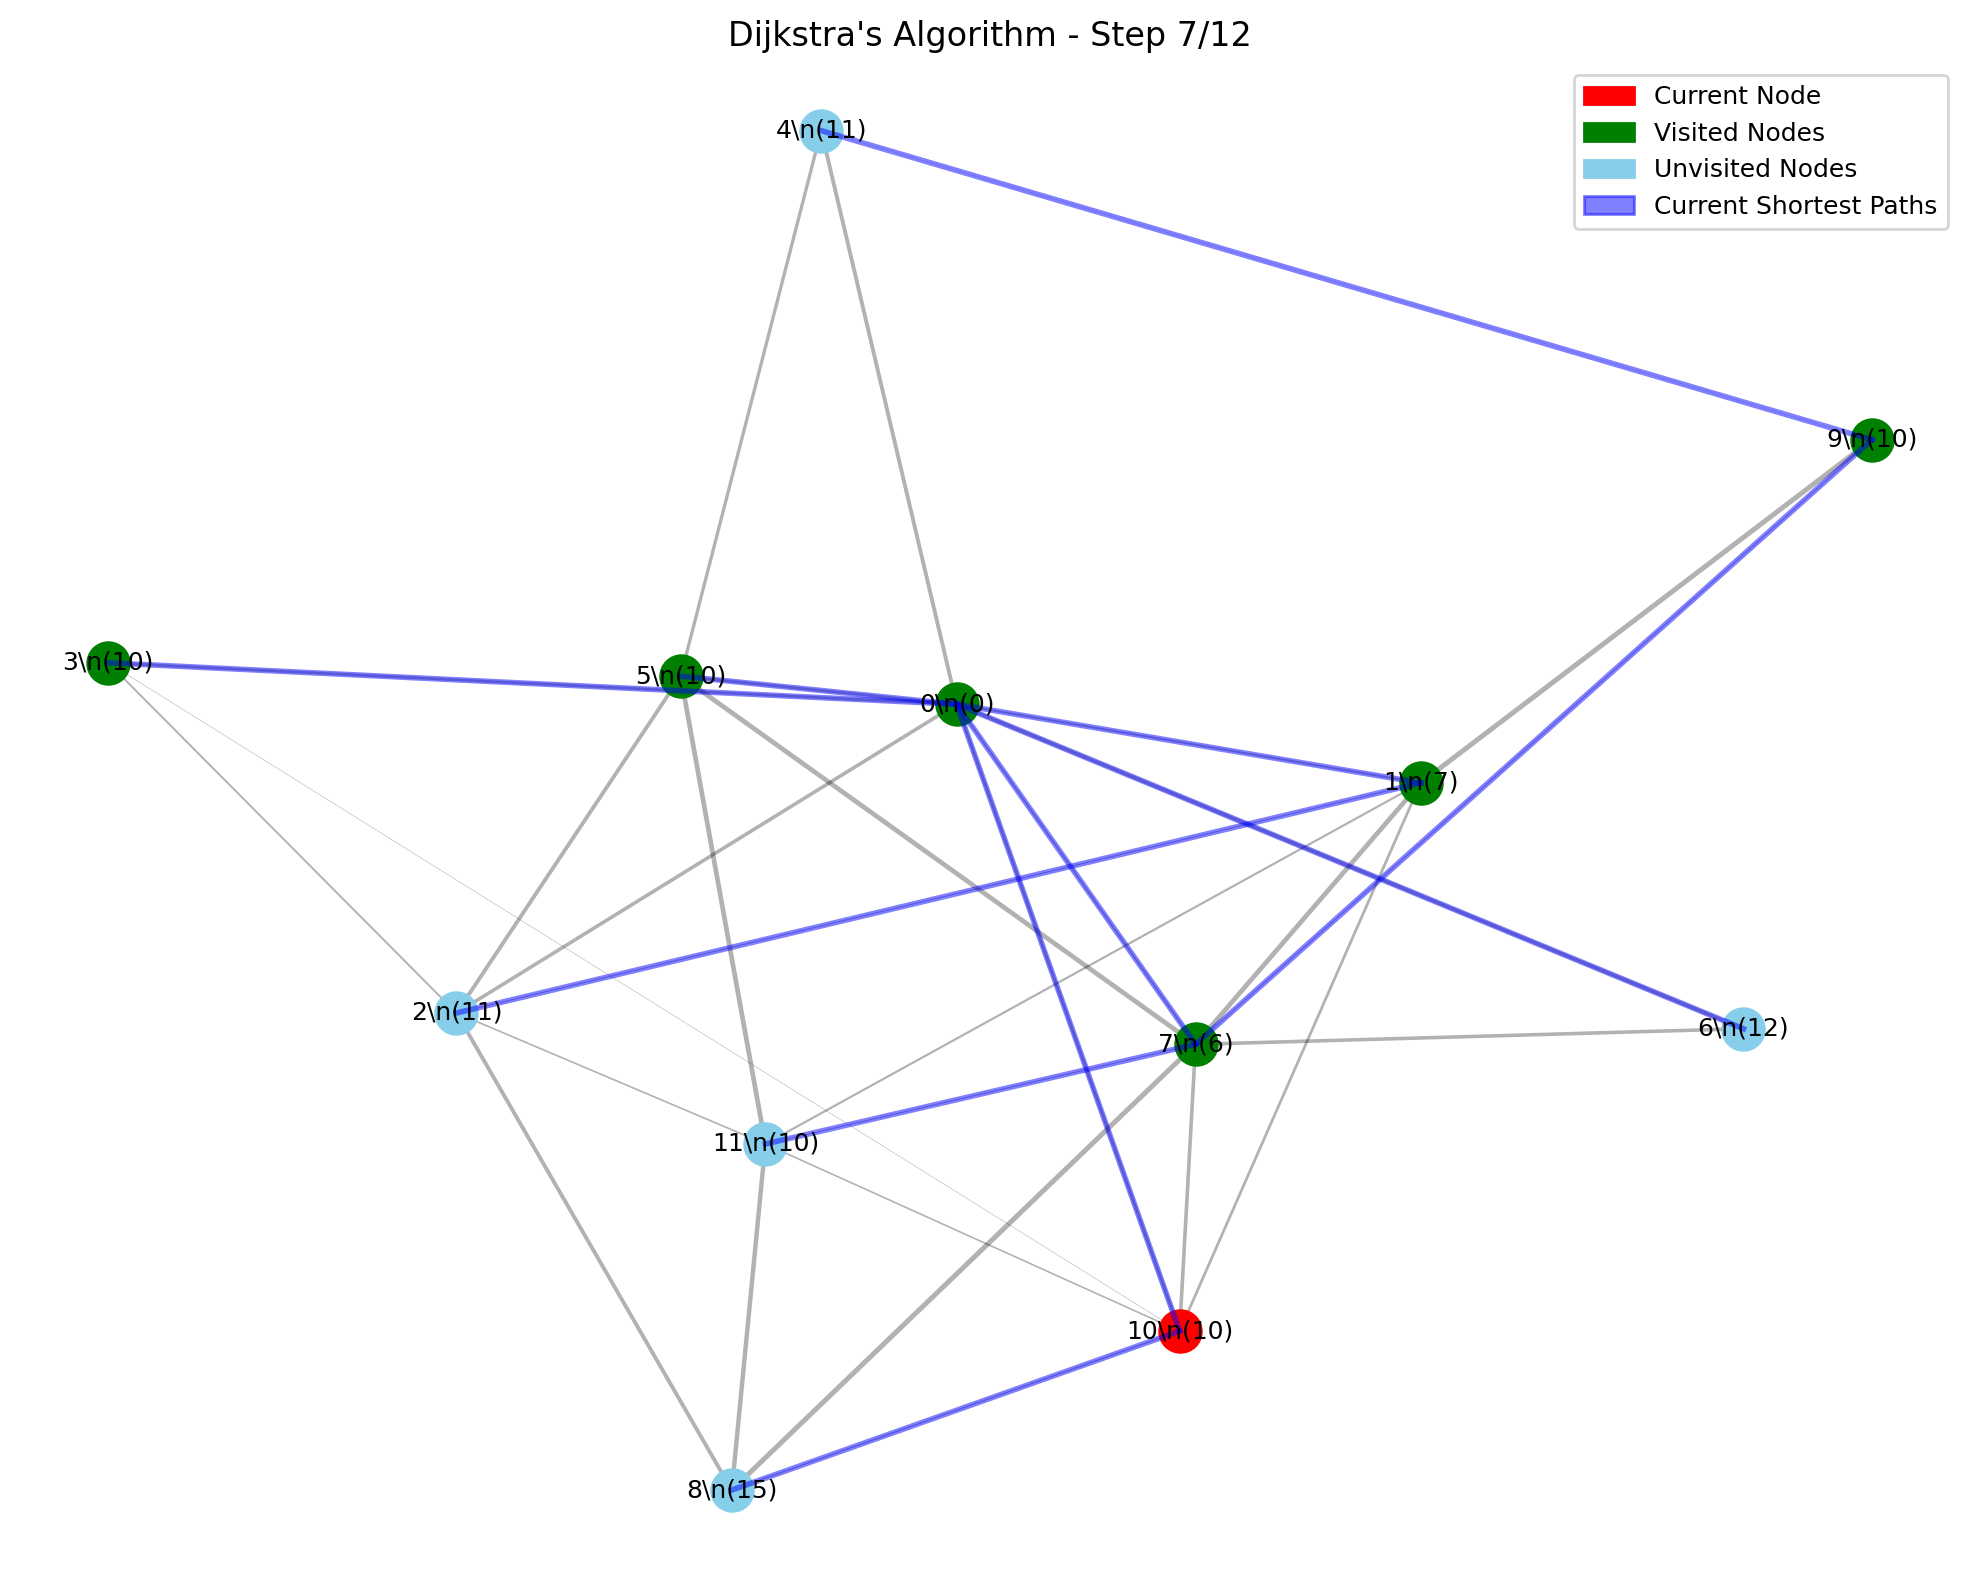
\includegraphics[width=0.75\textwidth]{report_images/dijkstra_snapshot.png}
  \caption{\textit{Dijkstra Algorithm Execution Snapshot}}
\end{figure}
The snapshot captures Dijkstra partway through execution and illustrates how shortest-path
estimates are progressively refined as vertices are processed in increasing order of distance.
In this frame, processed vertices form a growing frontier around the source, and only edges that
can improve tentative distances trigger updates. This behaviour highlights why Dijkstra performs
well on sparse graphs: useful relaxations are relatively localized, and the min-heap quickly
focuses work on the most promising vertices.


\phantomsection
\subsection{Comprehensive Empirical Comparison}

Comprehensive performance figures were generated directly by \texttt{main.py} as it
ran the empirical benchmarks. The plots display execution times in milliseconds averaged over five
independent runs for each configuration.
Together, these figures provide a layered interpretation: first by algorithm and density, then by
direct cross-algorithm comparison under fixed sparsity assumptions.

\begin{figure}[H]
  \centering
  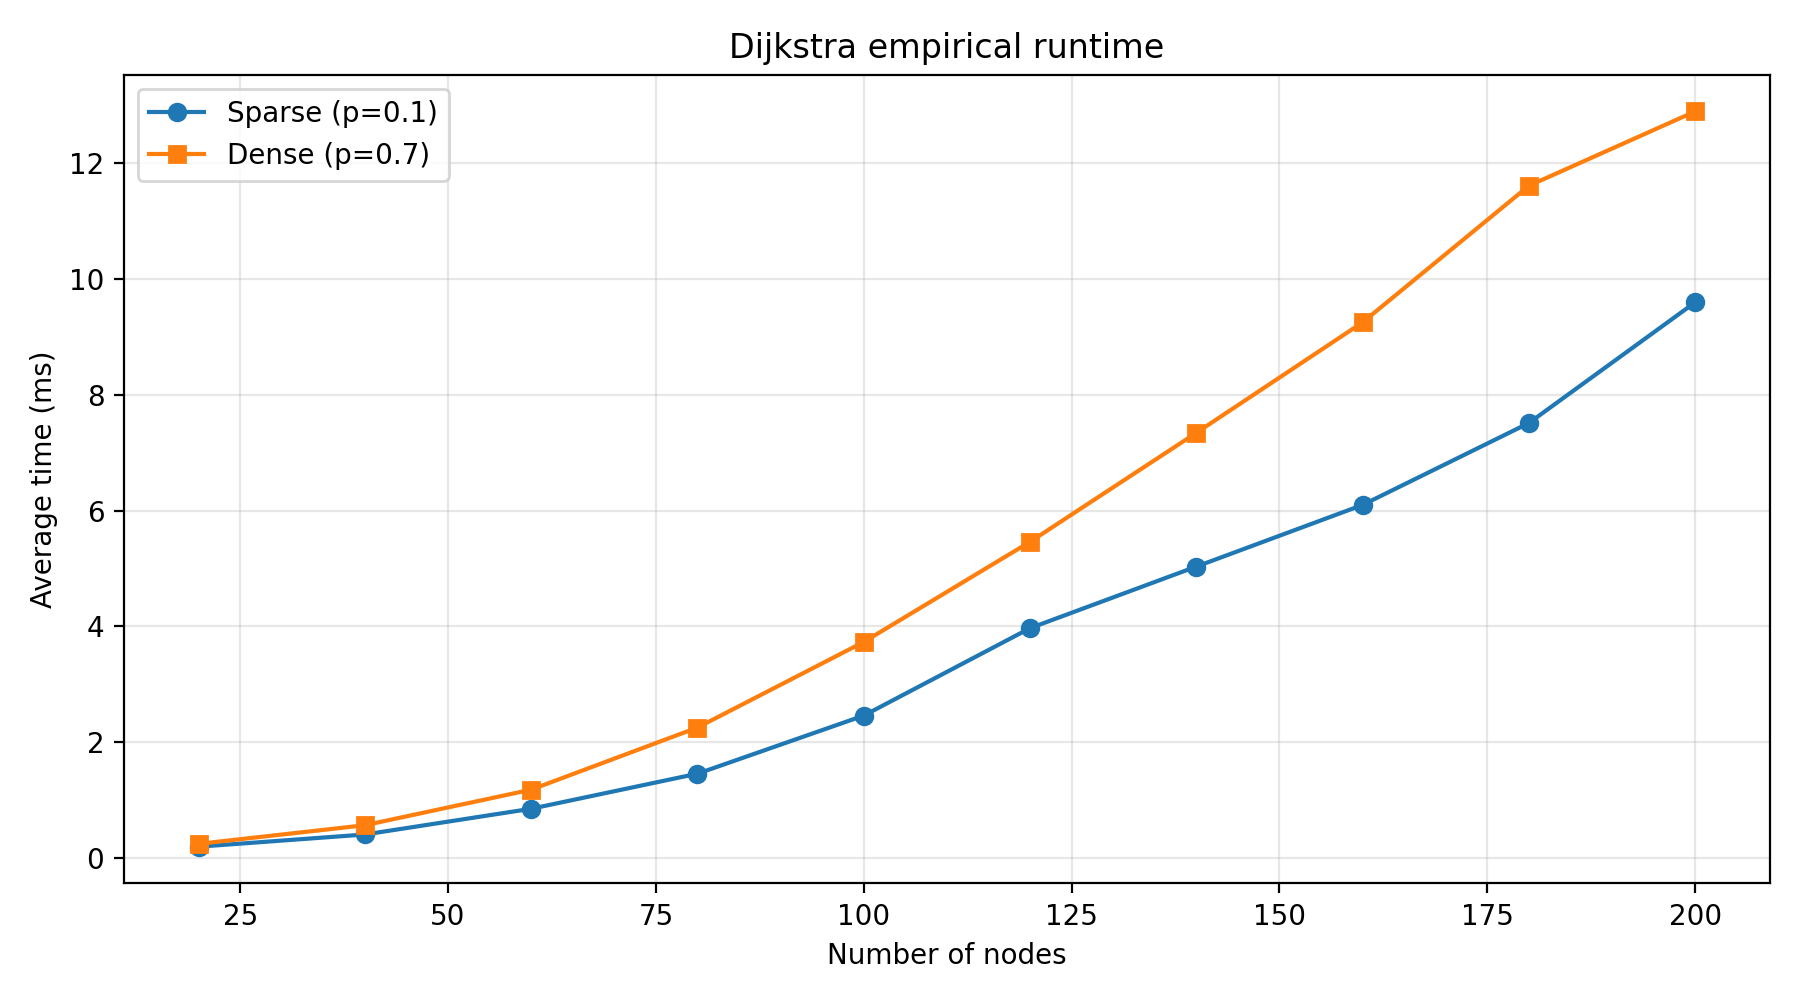
\includegraphics[width=0.85\textwidth]{report_images/dijkstra_sparse_dense.png}
  \caption{\textit{Dijkstra Runtime on Sparse and Dense Graphs.}}
\end{figure}
The Dijkstra plot shows a clear increase with graph size for both densities, but the dense
curve remains consistently above the sparse curve. This is expected because denser graphs induce
more candidate relaxations and more heap operations with meaningful updates.

\begin{figure}[H]
  \centering
  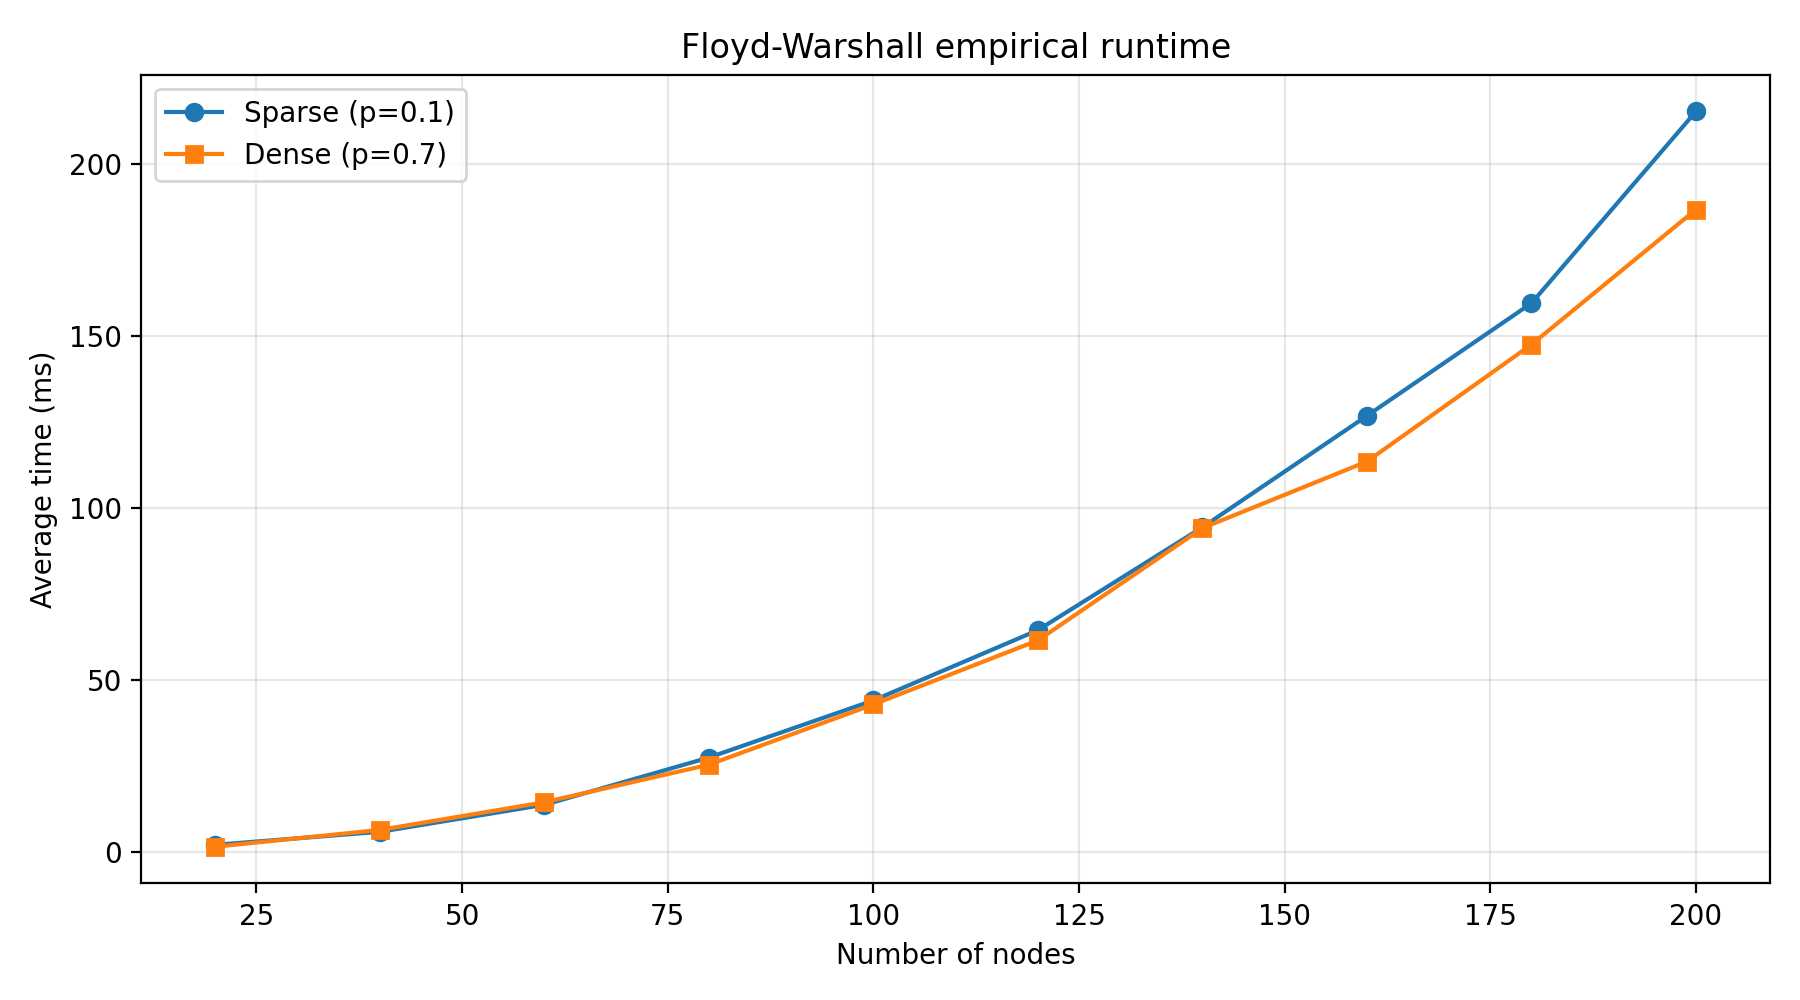
\includegraphics[width=0.85\textwidth]{report_images/floyd_sparse_dense.png}
  \caption{\textit{Floyd--Warshall Runtime on Sparse and Dense Graphs.}}
\end{figure}
The Floyd--Warshall curves are substantially steeper than Dijkstra's, reflecting the
$O(V^3)$ computational structure. The sparse and dense curves are closer to one another than in
Dijkstra, because Floyd--Warshall's dominant cost is the full matrix dynamic-programming update,
which depends primarily on $V$ and much less on edge count.

\begin{figure}[H]
  \centering
  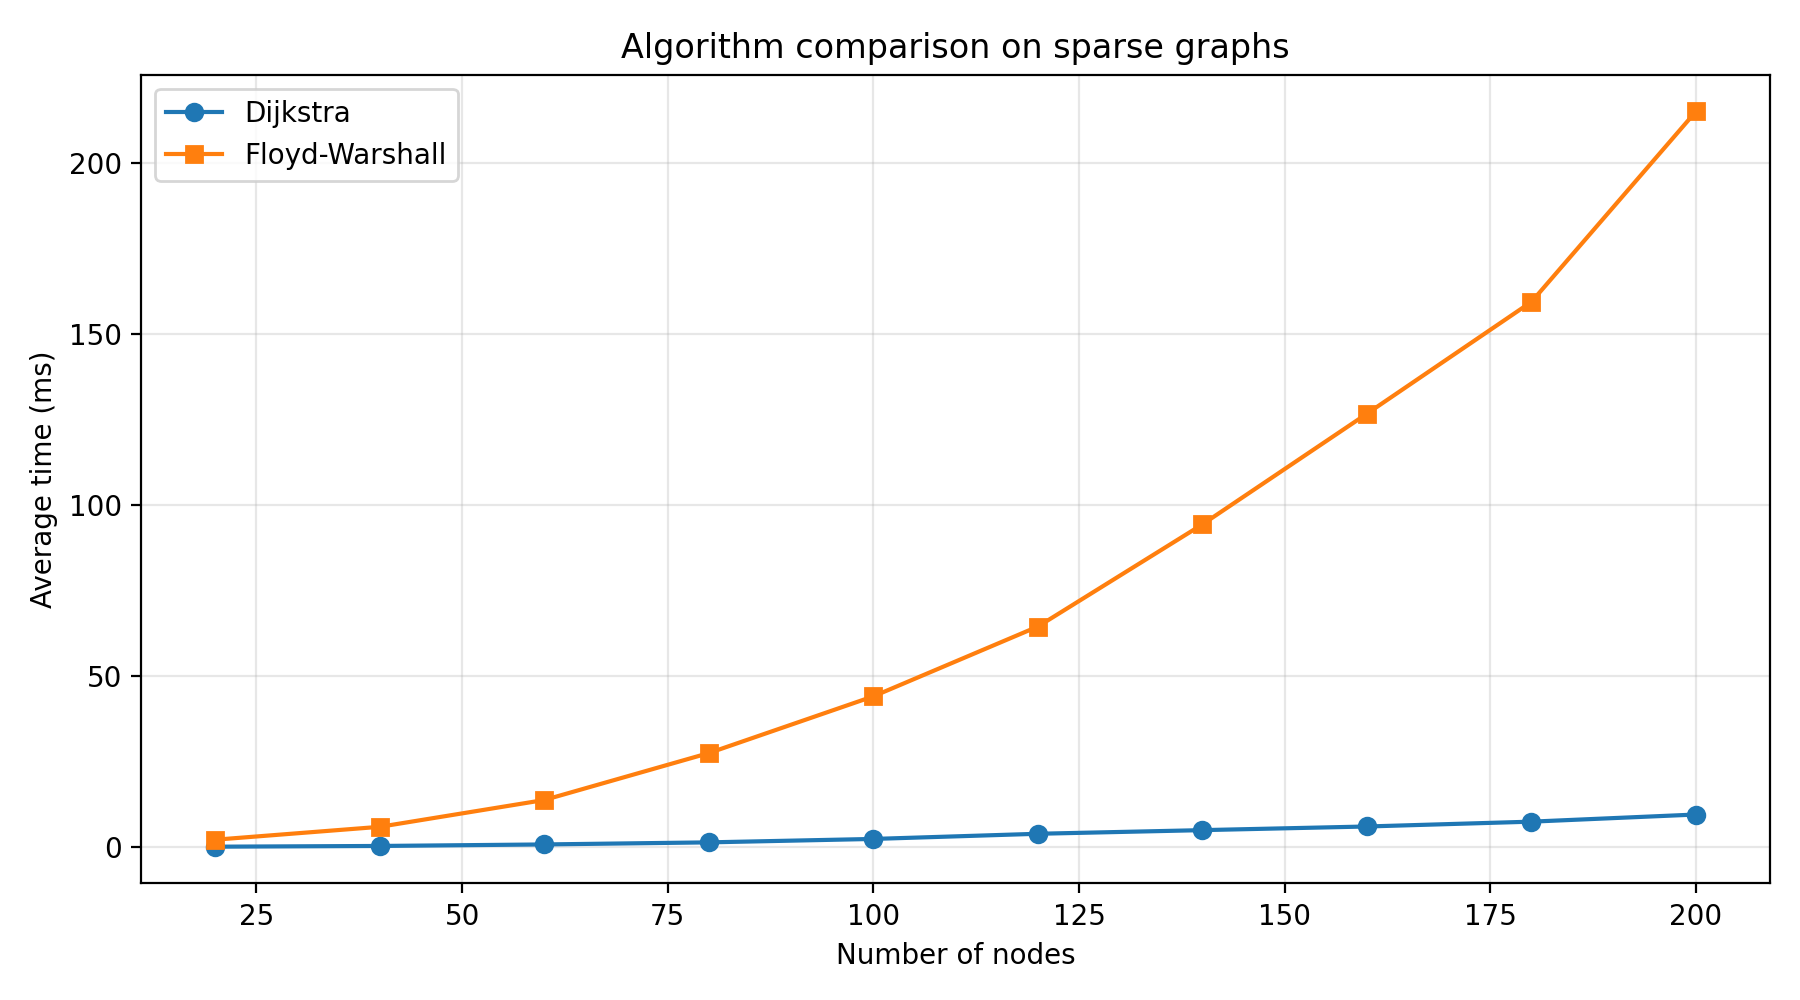
\includegraphics[width=0.85\textwidth]{report_images/comparison_sparse.png}
  \caption{\textit{Dijkstra vs Floyd--Warshall on Sparse Graphs.}}
\end{figure}
On sparse graphs, Dijkstra remains below Floyd--Warshall across all tested sizes, and the
gap widens as $n$ increases. This empirically confirms the practical advantage of source-focused
search over all-pairs preprocessing when the graph has relatively few edges.

\begin{figure}[H]
  \centering
  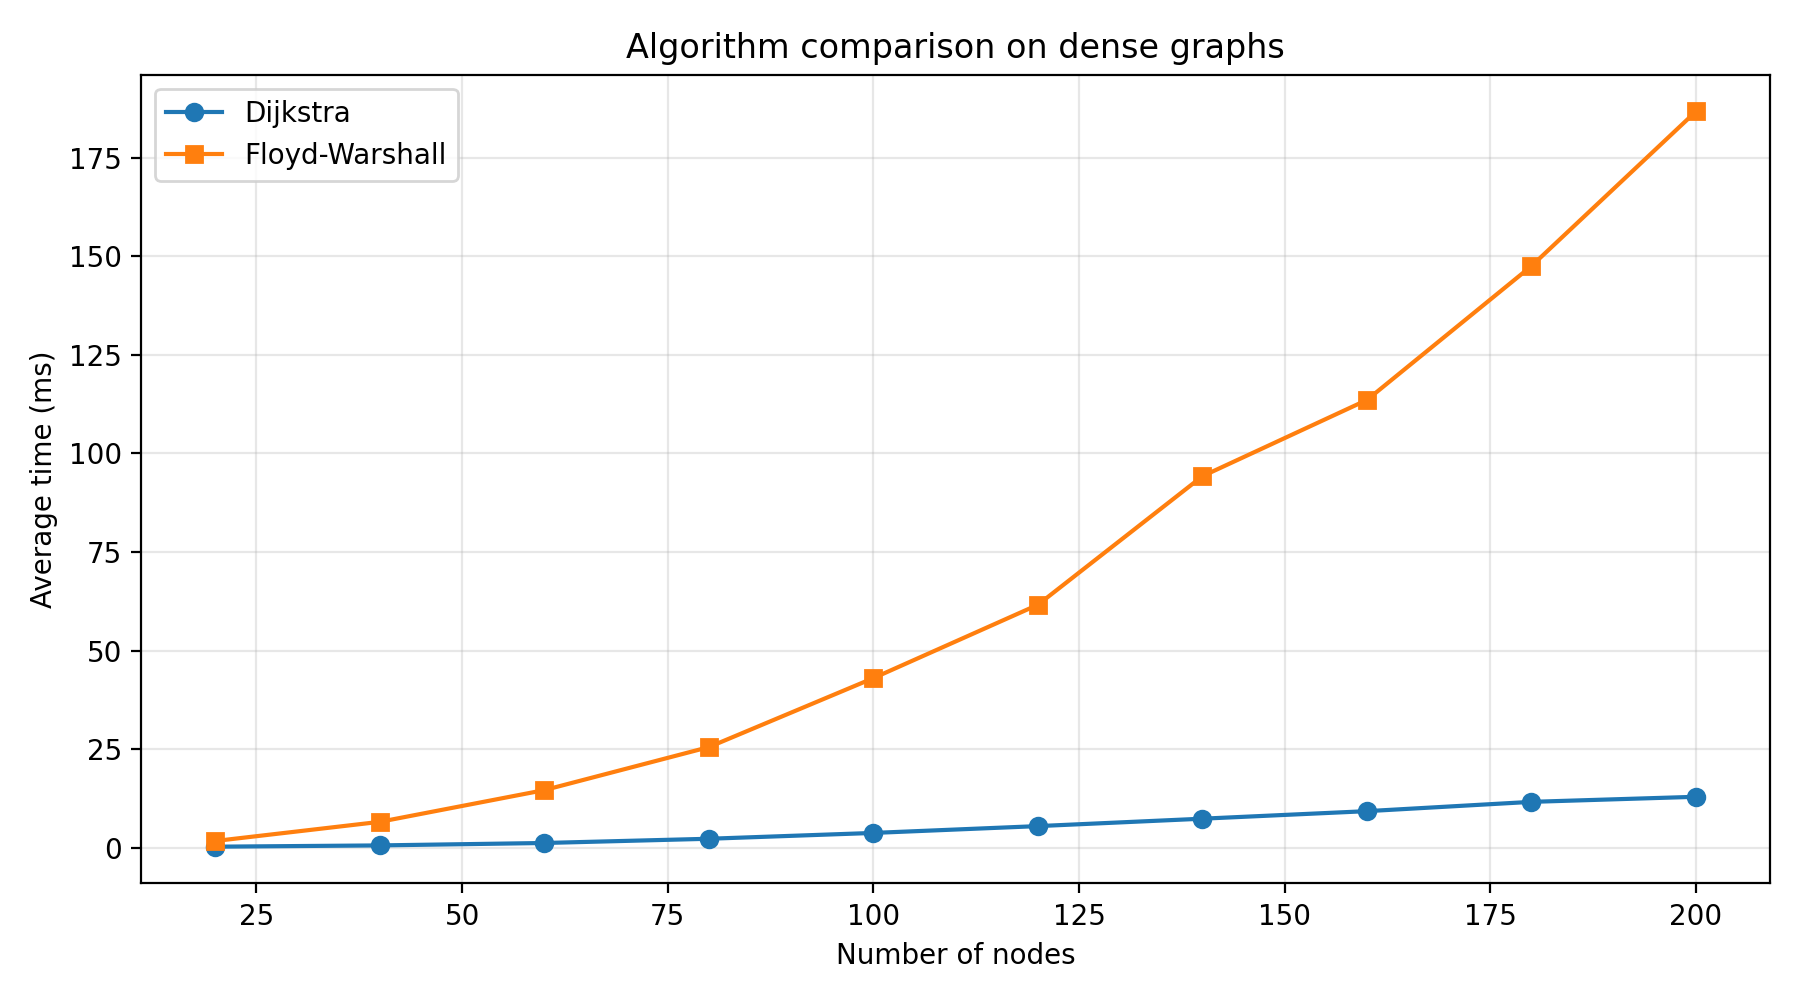
\includegraphics[width=0.85\textwidth]{report_images/comparison_dense.png}
  \caption{\textit{Dijkstra vs Floyd--Warshall on Dense Graphs.}}
\end{figure}
On dense graphs, both algorithms slow down, but Dijkstra still keeps a measurable lead in
this experimental range. The figure indicates that increased density narrows the practical gap,
yet does not invert it for sizes up to $n=200$ under the current implementation.

\begin{figure}[H]
  \centering
  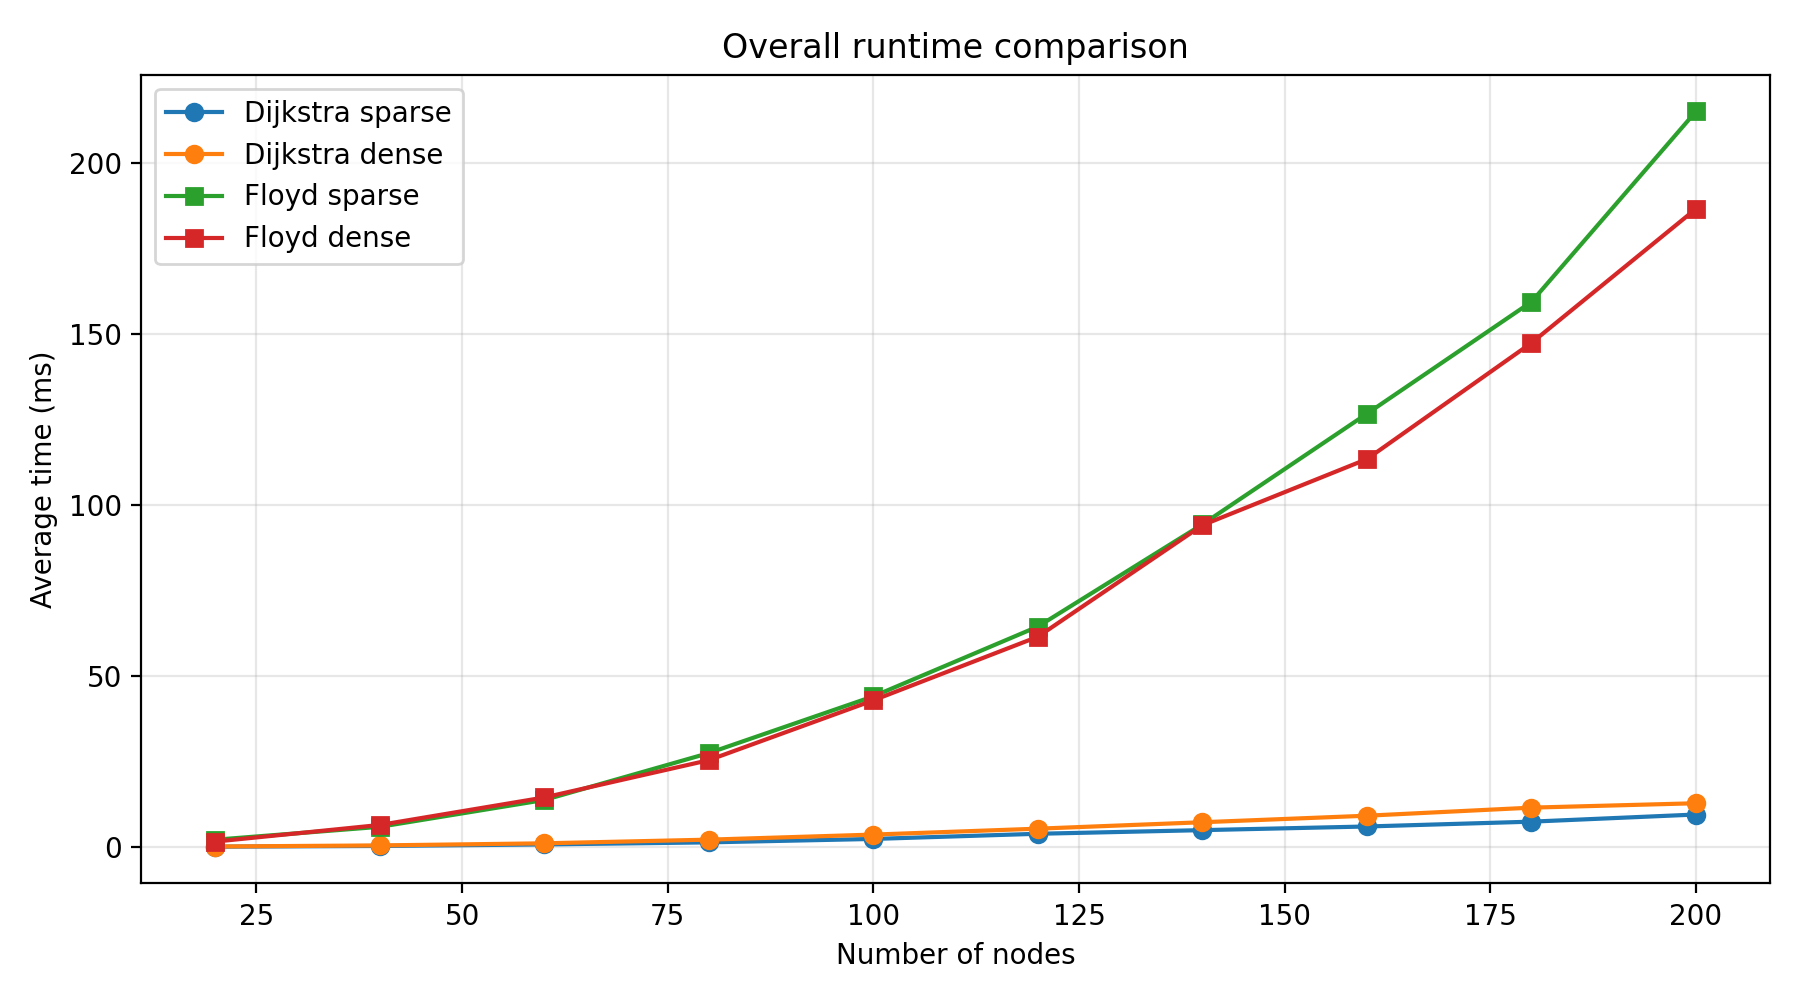
\includegraphics[width=0.85\textwidth]{report_images/overall_runtime.png}
  \caption{\textit{Overall Runtime Comparison.}}
\end{figure}
The unified chart consolidates all four experimental curves and makes trend comparison
immediate: the two Floyd--Warshall series form the upper envelope, while Dijkstra on sparse graphs
forms the lower envelope. This visual summary supports a straightforward decision rule for this
laboratory setting: prefer Dijkstra for single-source tasks, and reserve Floyd--Warshall for
use-cases where complete all-pairs distance information is required.

\newpage
\phantomsection
\section*{CONCLUSION}
\addcontentsline{toc}{section}{CONCLUSION}

The objectives of laboratory work 4 have been successfully completed. We have studied
the dynamic programming paradigm and its application to shortest-path problems, implemented both
Dijkstra's algorithm and the Floyd--Warshall algorithm in Python with careful attention to data
structures and efficiency, and conducted a rigorous empirical performance analysis comparing these
algorithms across a range of graph sizes and topologies.

Our empirical findings strongly confirm the theoretical predictions about algorithm complexity and
scaling behaviour. Dijkstra exhibits approximately $O((V+E)\log V) \approx O(V \log V)$ scaling on
sparse graphs---where edges are few and the heap rarely processes non-beneficial vertices and
$O(V^2 \log V)$ on dense graphs where edge scanning dominates. Floyd--Warshall demonstrates the predicted
consistent $O(V^3)$ behaviour regardless of edge density, a consequence of its uniform three-nested-loop
structure. These empirical observations validate decades of algorithmic analysis and provide concrete
evidence of the theoretical bounds in action.

The practical implications are equally clear. On sparse graphs, Dijkstra maintains a decisive speed advantage
over Floyd--Warshall across all tested sizes, with the gap widening as $n$ grows. This advantage stems directly
from Dijkstra's greedy focus on promising vertices via the priority queue: only reachable portions of the graph
are examined, whereas Floyd--Warshall blindly checks all $O(V^3)$ vertex triples. On dense graphs, both algorithms
slow significantly due to increased edge scanning, yet Dijkstra still outperforms Floyd--Warshall, a result that
holds throughout the tested range up to $n=200$.

For practitioners making algorithm selection decisions, the takeaway is straightforward. Dijkstra should be the
default choice for single-source shortest-path queries, offering superior performance especially on sparse graphs
and scaling gracefully with graph size. Floyd--Warshall is appropriate when complete all-pairs distance information
must be precomputed and then queried repeatedly, provided the precomputation cost is amortized over sufficiently
many queries. The choice is also influenced by additional factors: Floyd--Warshall correctly handles negative edge
weights (though our experiments used only positive weights), while Dijkstra requires non-negative weights. In systems
with memory constraints, Dijkstra's linear space usage is preferable to Floyd--Warshall's $O(V^2)$ distance matrix.

The generated performance charts provide clear visual evidence of these trade-offs. The temporal measurements, collected
using high-precision wall-clock timing and averaged over multiple runs, reveal both the expected asymptotic trends and
the constant factors that drive practical performance. The visualization snapshots and animated GIF files complement
the numerical results by showing how the algorithms explore graphs structurally different ways,Dijkstra radiating outward
from the source in a greedy frontier, Floyd--Warshall iteratively refining a complete distance matrix.


\newpage
\addcontentsline{toc}{section}{REFERENCES}
\phantomsection
\section*{REFERENCES}
\vspace{-2.5em}
\renewcommand{\refname}{}
\begin{thebibliography}{99}

\bibitem{github}
\textbf{P., I. (2026).} \textit{Analysis of Algorithms}. GitHub Repository.
\url{https://github.com/inap235/AALab}

\bibitem{geeks_dp}
GeeksforGeeks. (2025). \textit{Dynamic Programming}.
\url{https://www.geeksforgeeks.org/dynamic-programming/}

\bibitem{tutorialspoint_dp}
TutorialsPoint. (2025). \textit{Dynamic Programming (Data Structures \\& Algorithms)}.
\url{https://www.tutorialspoint.com/data_structures_algorithms/dynamic_programming.htm}

\bibitem{codingninjas_compare}
Coding Ninjas. (2025). \textit{Dijkstra's Algorithm vs Floyd-Warshall's Algorithm}.
\url{https://www.codingninjas.com/codestudio/library/dijkstras-algorithm-vs-floydwarshalls-algorithm}

\bibitem{cormen}
Cormen, T. H., Leiserson, C. E., Rivest, R. L., \& Stein, C. (2009).
\textit{Introduction to Algorithms} (3rd ed.). MIT Press.

\end{thebibliography}
\pagebreak
\end{document}
